\section{Plaintext encryption}

Encrypting plaintexts with a length less than or equal to the block size using a block cipher is effective.
This method can be expanded by employing multiple blocks with a split-and-encrypt approach, also known as Electronic CodeBook (ECB) mode.
\begin{figure}[H]
    \centering
    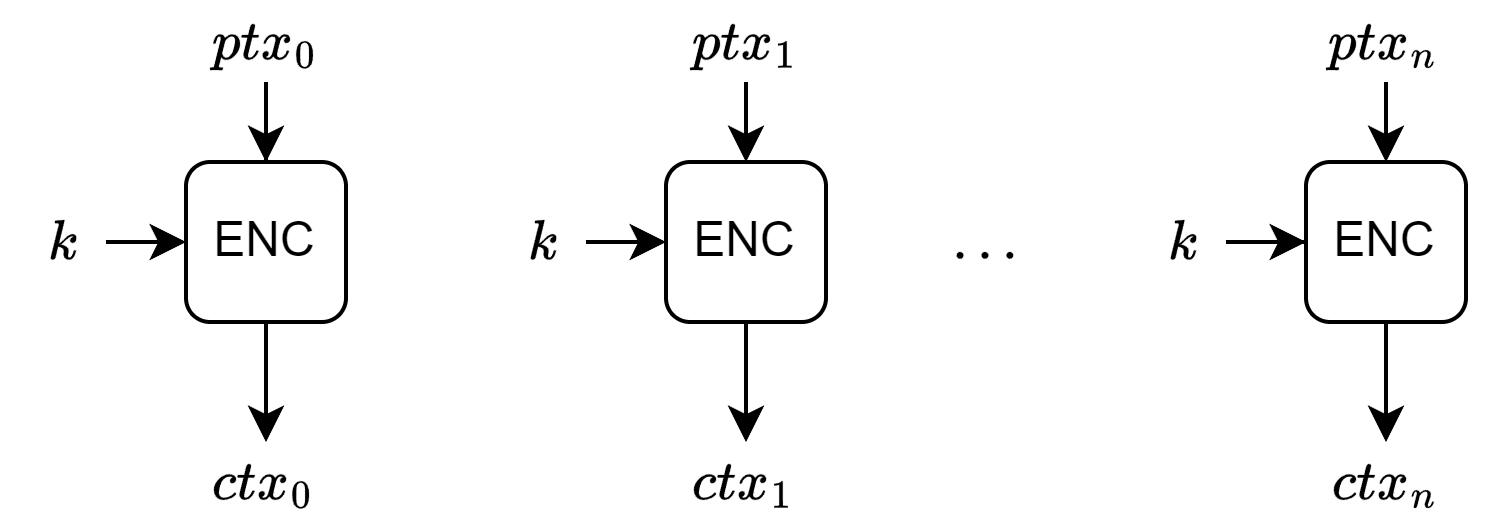
\includegraphics[width=0.55\linewidth]{images/ecb.png}
    \caption{ECB encryption mode}
\end{figure}
However, this technique becomes problematic when there is redundancy within plaintext segments, as the resulting ciphertext may still reveal patterns. 
This vulnerability arises from the deterministic nature of ECB encryption, where identical plaintext blocks produce identical ciphertext blocks, making it susceptible to certain cryptographic attacks.

To address the issue of pattern visibility in ciphertexts caused by redundancy in plaintext segments, we can employ a counter to differentiate the strings submitted to each block during encryption. 
This counter, unique for each block, helps mitigate the predictability inherent in traditional encryption modes.
\begin{figure}[H]
    \centering
    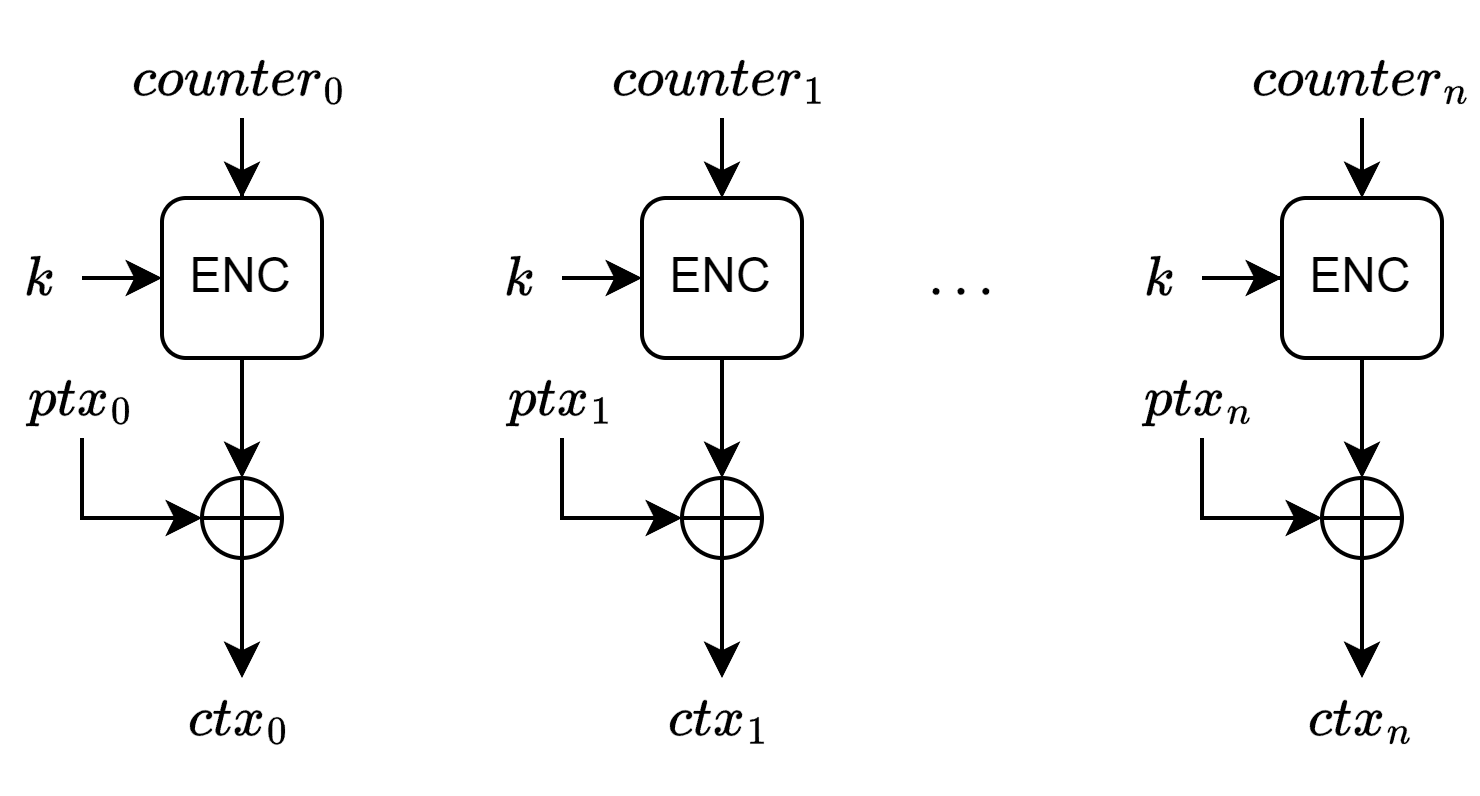
\includegraphics[width=0.55\linewidth]{images/ctr.png}
    \caption{CTR encryption mode}
\end{figure}
This method ensures that even if plaintext blocks are repeated, the resulting ciphertext blocks are different due to the unique counter values assigned to each block.

\subsection{Chosen-Plaintext Attacks}
Now, let's consider a scenario where the attacker has access to both the ciphertext and a portion of the plaintexts.
In this type of attack, the attacker is familiar with a series of plaintexts that undergo encryption, and their objective is to determine the specific plaintext being encrypted.

In an ideal situation, the attacker should not be able to distinguish between two plaintexts of equal length when provided with their encrypted versions.
Such scenarios frequently occur in contexts like managing data packets within network protocols and discerning between encrypted commands sent to a remote host.

The counter (CTR) mode of operation is vulnerable to Chosen-Plaintext Attacks (CPA) due to its deterministic encryption process.
To enhance security and achieve decryptable nondeterministic encryption, we can implement the following steps:
\begin{enumerate}
    \item \textit{Re-keying}: change the encryption key for each block using a mechanism like a ratchet, ensuring that each block's encryption is independent and unpredictable.
    \item \textit{Randomize the encryption}: introduce (removable) randomness into the encryption process by altering the mode of employing PRP. 
        This randomization enhances the unpredictability of the ciphertext, making it more resistant to cryptanalysis.
    \item \textit{Nonce usage}: utilize numbers used once (NONCEs) to introduce additional variability into the encryption process. 
        In the case of CTR mode, a NONCE is chosen as the starting point for the counter. 
        This NONCE can be public, adding an extra layer of unpredictability to the encryption.
\end{enumerate}
By implementing these measures, we can significantly enhance the security of the encryption process and mitigate vulnerabilities associated with deterministic encryption modes like CTR.

\paragraph*{Re-keying}
The term ratcheting is derived from the mechanical device called a ratchet, which allows movement in one direction while preventing backward movement. 
Similarly, in symmetric ratcheting, the encryption keys are ratcheted forward in a manner that prevents an attacker from decrypting past messages even if they compromise the current key.
\begin{figure}[H]
    \centering
    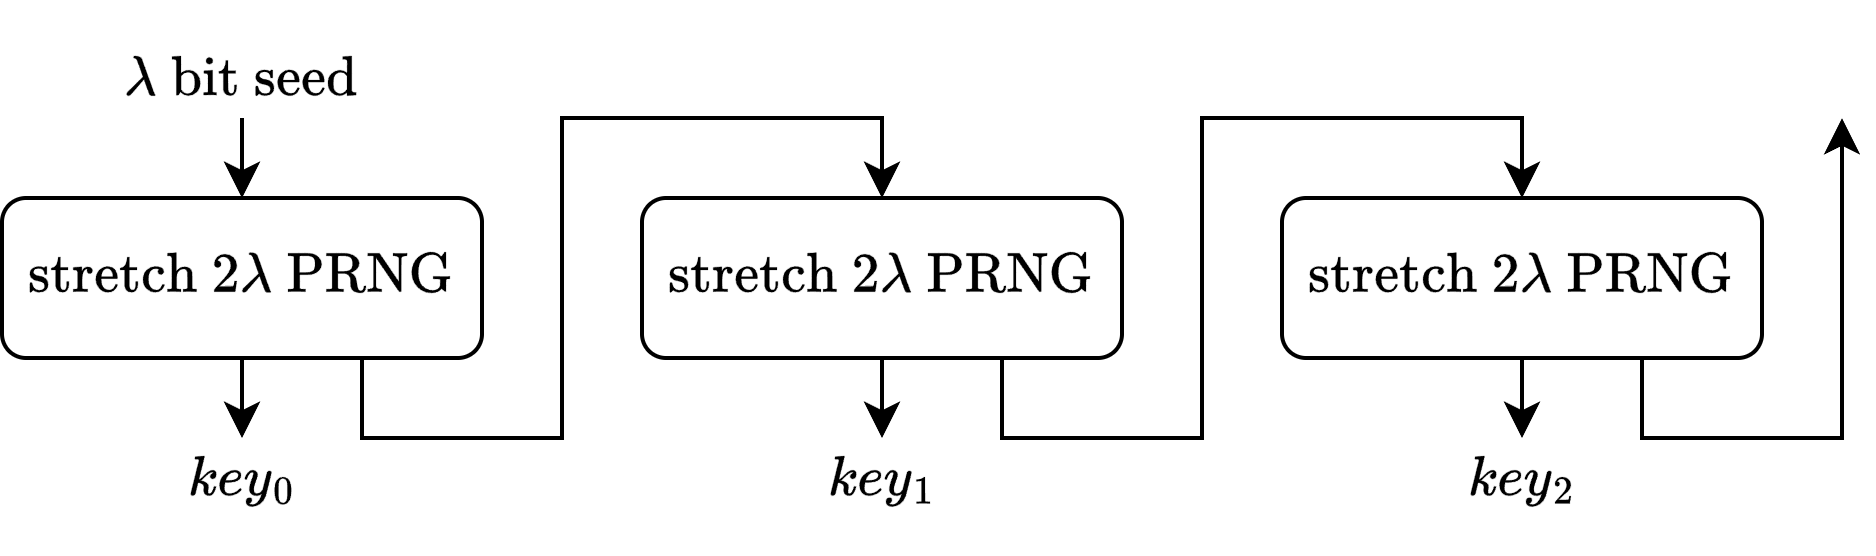
\includegraphics[width=0.75\linewidth]{images/ratchet.png}
    \caption{Ratcheting}
\end{figure}
Symmetric ratcheting ensures that even if an attacker manages to compromise the current encryption key, they cannot decrypt past messages or predict future messages due to the frequent key updates. 
This technique effectively limits the impact of key compromise and strengthens the security of encrypted communication over time.

\paragraph*{CPA secure encryption}
Secure encryption schemes are designed to withstand CPA by ensuring that an attacker cannot gain any useful information about the encryption key or plaintexts, even if they have access to ciphertexts for chosen plaintexts.
This is accomplished by utilizing the NONCE in conjunction with the CTR mode of operation.
\begin{figure}[H]
    \centering
    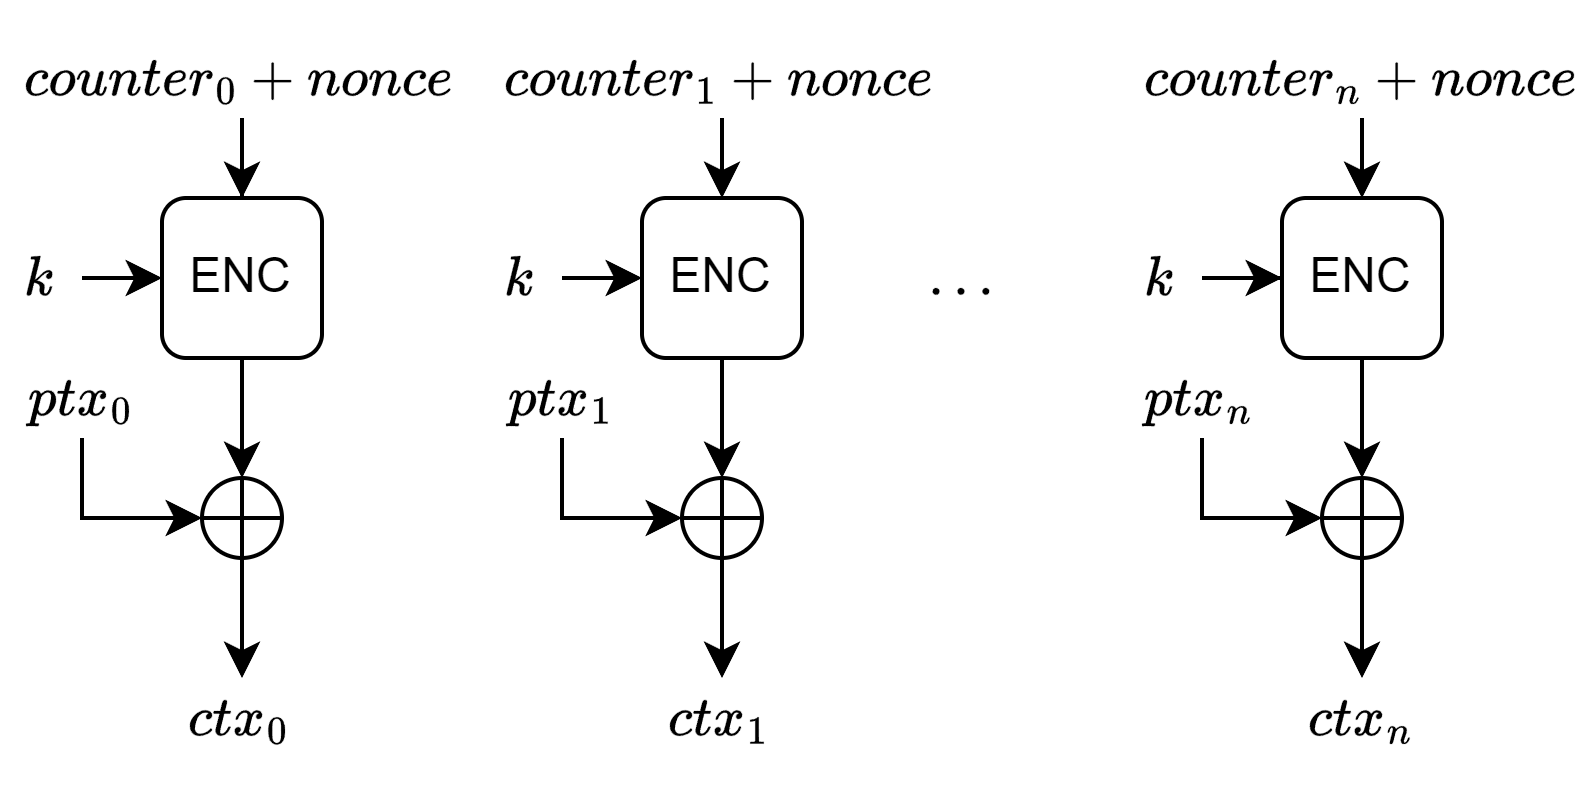
\includegraphics[width=0.75\linewidth]{images/sctr.png}
    \caption{Secure ctr}
\end{figure}